\documentclass[11pt,a4paper]{article}
% Generated from paper/manuscript.md by paper/build/build_latex.py -- edit the markdown, not this file.
\usepackage[utf8]{inputenc}
\usepackage[T1]{fontenc}
\usepackage{lmodern}
\usepackage[margin=2.5cm]{geometry}
\usepackage{graphicx}
\usepackage{microtype}
\usepackage[hidelinks]{hyperref}
\usepackage{setspace}
\usepackage{lineno}
\usepackage{caption}
\captionsetup{labelformat=empty,skip=2pt}
\setlength{\parskip}{6pt}
\setlength{\parindent}{0pt}
\date{}
\onehalfspacing
\linenumbers
\begin{document}
\title{Pre-treatment transcriptional prediction of sister-cell fate is dominated by fitness and limited by sister discordance}
\maketitle

\section*{Abstract}

\textbf{Background.} Cancer cells that survive treatment are often thought to be recognisable before treatment by their transcriptional state. Sister-cell lineage tracing makes this directly testable. In ReSisTrace, one sister is sequenced before treatment and the other is treated, so the fate of the treated sister labels the sequenced one. The design also includes an untreated control arm in which a cell's ``survival'' reflects only growth and recovery.

\textbf{Methods.} We used the ReSisTrace data (Kuramochi ovarian cancer cells; carboplatin, olaparib, NK cells and no-drug control; two replicates; 32,642 labelled pre-treatment cells). We trained classifiers directly on the lineage labels and evaluated them with lineage-grouped cross-validation, replicate hold-out and transfer between arms. We then measured how much of the predictive signal is shared with the control arm, estimated an upper bound on predictability from 3,477 pairs of sisters that were both sequenced before treatment, and tested for confounding by sequencing depth, cell cycle and inferred copy-number subclones. Two independent lineage-tracing data sets, the TCGA ovarian cancer cohort and a cohort of 11 patients sampled before and after neoadjuvant chemotherapy served as external checks.

\textbf{Results.} A logistic model on 50 principal components predicted the sister's fate with AUROC 0.72--0.75 in the drug arms (label-permutation p $<$ 0.01). On the olaparib arm, under the same balanced protocol, this was well above the AUROC of about 0.50--0.60 reported for existing drug-response predictors, and neither tuning, pooling arms, gradient boosting, a graph neural network with sister-pair pretraining nor embeddings from a single-cell foundation model improved on it (graph network 0.70--0.73 across three seeds; Geneformer 0.67--0.68). However, a model trained only on the untreated control arm predicted the drug-arm labels almost as well (AUROC 0.70--0.73). With training size matched, the drug-specific gain over this fitness model was 0.014--0.025 AUROC (95\% confidence intervals excluding zero in every drug arm) and fell to 0.003 for NK cells once depth and mitochondrial content were removed (95\% CI $-$0.010 to 0.016). Beyond the fitness axis, pre-resistant cells showed lower E2F, mitotic-spindle and MYC-target expression. A label-free score of how typical a cell's state is reached AUROC 0.63--0.70 on its own. Sister discordance alone cost about 0.09--0.12 AUROC. Inferred copy-number subclones did not explain the signal. In two external data sets, clone size predicted lineage survival far better than expression, and ReSisTrace models transferred at or near chance. No derived signature was associated with outcome in TCGA ovarian tumours after correction for multiple testing, and in 11 patients sampled before and after neoadjuvant chemotherapy the drug signatures were not enriched in the cells that persisted, while the fitness signature was depleted.

\textbf{Conclusions.} In this system, most of what a pre-treatment transcriptome says about a sister's survival is generic fitness rather than drug-specific tolerance, and even a perfect model of the sequenced cell would be limited by the imperfect similarity of sisters. The fitness state does not appear to be what selects cells in treated patients. Untreated controls and sister-based ceilings should accompany claims that pre-existing states predict drug tolerance, and we provide them as a small reusable package.

\textbf{Keywords:} drug tolerance; lineage tracing; single-cell RNA-seq; sister cells; cell fate prediction; non-genetic resistance

\section*{Introduction}

Resistance to cancer therapy does not always need a mutation. Sharma et al. (2010) described a small, reversibly drug-tolerant subpopulation in several drug-sensitive cancer cell lines. These cells showed more than 100-fold reduced drug sensitivity, depended on IGF-1 receptor signalling and a KDM5A-dependent chromatin state, and were entered and left at low frequency by individual cells. Persisters of this kind can later acquire a variety of genetic resistance mechanisms (Hata et al., 2016; Ramirez et al., 2016), which makes the question of how cells enter the tolerant state clinically important. Non-genetic resistance has since been reviewed as a broad class of adaptive mechanisms (Marine et al., 2020; Soragni et al., 2025).

A central question is whether survivors were already different before the drug was given. Several lines of work suggest that, at least in part, they were. In melanoma, rare cells expressing a set of resistance markers at high levels, at frequencies of about 1 in 50 to 1 in 500, were more likely to become resistant, and drug exposure then converted this transient state into a stable one (Shaffer et al., 2017). MemorySeq showed that gene expression fluctuations can persist for several divisions within otherwise homogeneous clonal populations, and that such rare subpopulations are associated with proliferation under anti-cancer drugs (Shaffer et al., 2020). Rewind combined barcoding with RNA FISH to trace resistant fates in BRAF-mutant melanoma back to rare drug-naive precursors, at frequencies of roughly 1:1,000 to 1:10,000 (Emert et al., 2021). FateMap found that the type of resistant clone a cell forms is largely set by differences present before drug addition (Goyal et al., 2023). Long-lived fluctuations in gene expression in untreated melanoma cells also predicted later resistance, and modulating them with a PI3K inhibitor before targeted therapy reduced resistance (Harmange et al., 2023). Tracing the same barcoded melanoma clones through six treatments in parallel, Schaff et al. (2026) found that clones resistant to one treatment were more likely to resist others, and that high CD44 expression before treatment marked multi-treatment resistance. From time-lapse lineages of cisplatin-treated cells, Iyer et al. (2025) inferred that survival is largely biased by cell states that exist before the drug and are inherited over two to three generations, with further modulation by the drug itself.

Other studies point the other way. In patient-derived colorectal cancer models, barcoding and mathematical modelling fitted a scenario in which all cells, not a rare subpopulation, have an equal capacity to enter a diapause-like persister state (Rehman et al., 2021). In colorectal cancer organoids followed through sequential treatments, oxaliplatin resistance arose from transient phenotypic plasticity rather than stable clonal selection (Oliveira et al., 2025). Live-cell imaging has long shown that fate after a death signal is only partly heritable. In TRAIL-induced apoptosis, differences in protein state are passed from mother to daughter, but sister cells soon become no more similar to each other than random pairs (Spencer et al., 2009). In colon cancer cells treated with chemotherapy, survivors and dying cells reached similar p53 levels, and the probability of death depended on the dynamics of p53 rather than on a fixed threshold (Paek et al., 2016). These results suggest that some of a cell's fate is decided after treatment begins, which limits what any pre-treatment measurement can predict.

Expressed lineage barcodes read out by single-cell RNA sequencing have made it possible to link the state of a cell to the fate of its relatives at scale (Wagner and Klein, 2020). In haematopoiesis, Weinreb et al. (2020) used this approach to locate states of primed fate potential, and their analysis of sister cells revealed intrinsic fate biases that single-cell RNA sequencing could not detect. CoSpar showed that such lineage data can reveal early fate biases even when sparse (Wang et al., 2022). In cancer, SPLINTR found that clonal dominance in acute myeloid leukaemia is a heritable, cell-intrinsic property (Fennell et al., 2022). Watermelon linked lineage, proliferation and transcriptional state in PC9 lung cancer cells under osimertinib and showed that cycling and non-cycling persisters arise from different lineages (Oren et al., 2021). ClonMapper identified subpopulations of a leukaemia cell line with distinct clonal compositions, transcriptional signatures and chemotherapy survival (Gutierrez et al., 2021). In triple-negative breast cancer, lineage tracing under the EGFR inhibitor afatinib identified a rare pre-existing subpopulation with high IGFBP2 expression that was sufficient to confer tolerance (Pellecchia et al., 2024). Most of these designs, however, label whole clones, so a surviving clone may contain cells in quite different states, and clone size itself affects whether a lineage is observed again.

ReSisTrace addresses this by letting barcoded cells divide once before splitting sisters between sequencing and treatment (Dai et al., 2024). Each sequenced cell is labelled by its own sister's fate rather than by a clone. The authors noted that Watermelon identified resistance-associated patterns only during, not before, treatment. They also included an untreated control arm that reproduces the synchronisation, splitting and re-plating steps, precisely to assess the confounding effect of experiment-specific growth fitness. In that control arm they found transcriptomic differences between cells whose sisters survived and those whose sisters did not, and they concluded that pre-resistance signals should be assessed against this experimental fitness signal (Dai et al., 2024). Their analysis was based on differential expression signatures, which they then used to predict pre-sensitising drugs. They did not build classifiers or report how well a cell's fate could be predicted.

Computational tools for single-cell drug response have mostly been built around a different problem. scDEAL transfers drug-response knowledge from bulk cell-line data to single cells (Chen et al., 2022). SCAD does the same with adversarial domain adaptation and argues that this can reveal pre-existing subpopulations with different sensitivities (Zheng et al., 2023). Beyondcell scores cells against collections of drug signatures (Fustero-Torre et al., 2021), and CaDRReS-Sc uses a recommender system to predict response from single-cell signatures (Suphavilai et al., 2021). A recent benchmark of nine such methods used the ReSisTrace olaparib arm as ground truth (Shen et al., 2026). When pre-treatment cells were compared with post-treatment survivors, the best method reached a mean AUROC of 0.869. When only pre-treatment cells were used with sister-derived labels, most methods fell to 0.50--0.55 and the best, scDEAL, to about 0.6. The authors concluded that current models capture drug-induced changes rather than intrinsic resistance.

These findings leave three questions open, and we address them here. First, how much signal about a sister's fate does the pre-treatment transcriptome actually contain when a model is trained directly on the lineage labels? Second, how much of that signal is specific to the drug, as opposed to the growth and recovery advantage that Dai et al. (2024) anticipated with their control arm? Third, what is the best performance one could hope for, given that the label belongs to a different cell? We quantify each of these on the ReSisTrace data, test the main confounders, and check whether the signal generalises to other lineage-tracing systems and to patients.

\section*{Results}

\subsection*{The pre-treatment state predicts a sister's fate, reproducibly (Fig. 1, Fig. 2)}

We used the authors' processed labels. After excluding 4,369 cells without a detected lineage label, 32,642 pre-treatment cells remained: 29,540 pre-sensitive and 3,102 pre-resistant. These counts match the original report exactly. Pre-resistant cells made up 7.8--11.2\% of labelled cells in the drug arms and 14.7--14.9\% in the control arm (Fig. 1b). Cells that shared lineage barcodes formed 29,437 families, all of them label-concordant. Every evaluation kept whole families on one side of the split.

An L2-regularised logistic regression on 50 principal components reached pooled out-of-fold AUROCs of 0.747 (carboplatin), 0.744 (olaparib), 0.723 (NK) and 0.708 (control) (Fig. 2a). Retraining the logistic model on labels permuted at the family level within each sample gave AUROCs around 0.50 (for gradient boosting the shuffled controls were higher, as described below). In an exact permutation test with 100 refits, no permuted AUROC reached the observed value in any arm (null mean 0.500--0.501, s.d. 0.015--0.019; p $<$ 0.01, the smallest value attainable). Training on one replicate and testing on the other gave 0.70--0.76 (Fig. 2b). Restricting the analysis to cells without a sister in the pre-treatment sample, as the original authors did for their differential expression, gave slightly higher values (carboplatin 0.754, olaparib 0.753, NK 0.737, control 0.720).

More elaborate models did not help. Nested tuning of the regularisation strength and number of components changed AUROC by at most 0.002, and adding labelled cells from the other arms by at most 0.004. Gradient boosting was slightly worse, whether it used components plus covariates (0.70--0.73) or 2,000 highly variable genes (0.70--0.73), and linear models on the 2,000 genes were worse still (0.63--0.66).

Under the protocol of the published benchmark (olaparib, all pre-resistant cells against an equal number of randomly drawn pre-sensitive cells, three draws), the same logistic model reached 0.739--0.756 with ordinary five-fold cross-validation and 0.734--0.747 with lineage-grouped folds (Fig. 2c). Grouping by lineage lowered AUROC by less than 0.01. The gap to the 0.50--0.60 reported by Shen et al. (2026) is therefore not due to sister cells leaking between training and test folds. It reflects training directly on the lineage labels rather than transferring from bulk drug-response data. Table S20 sets out the inputs, training signal, labels and protocol behind each value; the published methods were not rerun here.

A model that used only sequencing depth, number of detected genes, mitochondrial fraction and cell-cycle scores reached 0.59--0.65 (Fig. 2a). Pre-resistant cells had lower UMI counts than pre-sensitive cells in every arm, including the control (Fig. 1c). To check that the main signal is not a technical artefact, we regressed cell-cycle scores alone, or cell-cycle scores together with log counts, log detected genes and mitochondrial fraction, out of the expression matrix before PCA. Removing cell cycle changed nothing (0.707--0.748). Removing depth and mitochondrial content as well lowered AUROC modestly (carboplatin 0.723, olaparib 0.727, NK 0.680, control 0.704).

\subsection*{Most of the signal is shared with the untreated control (Fig. 3)}

If the pre-treatment state encoded tolerance to a particular drug, models should transfer poorly between mechanistically unrelated treatments, and a model trained on the untreated control should transfer worst. Neither was the case. All twelve cross-arm transfers gave AUROC 0.69--0.74 (Fig. 3a). The control-trained model scored 0.725 on carboplatin, 0.713 on olaparib and 0.697 on NK labels, within 0.02--0.03 of models trained on those arms. Drug-arm models, in turn, predicted the control labels with 0.69--0.70, close to the control model's own 0.708.

Drug-arm and control-model scores were strongly correlated (Spearman 0.80--0.82). Adding the drug score to a logistic model that already contained the control-model score still improved fit in every arm (likelihood-ratio p $<$ 10$^-$$^2$$^5$). The drug-specific component was therefore real, but it was small. The drug score residualised on the control score reached AUROC 0.60--0.63, and within quintiles of the control score 0.64--0.66 (Fig. 3b). The control arm has fewer labelled cells (4,183) than the drug arms (8,942--10,123), so we also trained drug models on random sets of whole families of the same size, repeated ten times, and put a paired family-bootstrap confidence interval on the difference (Methods). The drug-specific advantage was then 0.014 for carboplatin (95\% CI 0.001--0.026), 0.025 for olaparib (0.012--0.039) and 0.017 for NK (0.003--0.031) (Fig. 3c, Table S19). The spread across the ten training subsets was small (s.d. 0.003--0.004). The gain was essentially unchanged after removing cell cycle (0.014, 0.025, 0.014). After removing depth and mitochondrial content as well, it was 0.012 for carboplatin ($-$0.001 to 0.025), 0.021 for olaparib (0.008--0.035) and 0.003 for NK ($-$0.010 to 0.016). For NK cells, therefore, nothing drug-specific could be distinguished from zero. The result did not depend on how expression was represented. We repeated the analysis with Harmony-corrected components (batch = sample; Korsunsky et al., 2019), with principal components of analytic Pearson residuals, a count-based alternative to log-normalisation (Lause et al., 2021), and with the latent space of scVI, which models library size and sample explicitly (Lopez et al., 2018). We also replaced the principal components with 768-dimensional cell embeddings from Geneformer, a transformer pretrained on 104 million human single-cell transcriptomes and continually pretrained on about 14 million cancer transcriptomes (Theodoris et al., 2023; Chen et al., 2026). The foundation model did not extract more signal than 50 principal components: it reached 0.671--0.683 in the drug arms, below the 0.723--0.747 of the linear model, and its fitness model still explained most of that (0.634--0.663), leaving a size-matched gain of 0.017--0.030. Across all four alternative representations, drug-arm models reached 0.671--0.746, the control-trained model 0.634--0.722 on the same labels, and the size-matched drug-specific gain (simpler five-repeat estimate) was 0.013--0.032 (Table S17).

\subsection*{A label-free measure of typicality recovers much of the signal (Fig. S1)}

While checking the shuffled-label controls, we noticed that gradient boosting trained on shuffled labels still scored above chance on the true labels (AUROC 0.56--0.58 in six refits on the olaparib and carboplatin arms; 0.56 with principal components alone), although the shuffled labels were uncorrelated with the true ones (|r| $<$ 0.01). Logistic regression trained on the same shuffled labels scored 0.47--0.54. This led us to a simple label-free score: the mean distance from a cell to its 15 nearest neighbours in principal-component space within its own sample. Pre-resistant cells lay in denser, more typical regions of state space. Density alone separated the classes with AUROC 0.70 (carboplatin), 0.69 (olaparib), 0.63 (NK) and 0.67 (control), essentially unchanged within single samples and after removing cell cycle, depth and mitochondrial content (0.63--0.69). It correlated with the supervised PCA-logistic score (Spearman 0.54--0.70). Much of what the supervised models learn is therefore available without any labels: cells whose sisters are recovered, with or without treatment, tend to be in common states, and cells in unusual states tend to lose their sisters. The control arm shows the same pattern as the drug arms, which fits a fitness effect. It also means that shuffled-label controls for flexible models should not be assumed to sit at 0.5, and each model should be compared with its own null. The effect is specific to this design: in the two external lineage-tracing data sets, where labels belong to whole clones rather than to a sister, the same score reached only 0.53 and 0.57 (Table S13). Density therefore tracks whether a cell's sister is recovered, not whether a clone is re-sampled.

\subsection*{What distinguishes the shared and drug-specific components (Fig. 4a)}

We compared pre-resistant with pre-sensitive cells within each sample and combined replicates. This gave 1,128--1,265 replicate-consistent differentially expressed genes in the drug arms and 639 in the control arm. More than a thousand genes per drug arm were shared with the control contrast. Only 57 (carboplatin), 221 (olaparib) and 140 (NK) were significant beyond it. Mitochondrial transcripts ranked near the top in every arm, including the control, in line with the depth difference noted above. We excluded them, together with ribosomal genes, from all signatures.

Hallmark gene-set enrichment of the control contrast showed higher MYC-target, mTORC1, E2F and fatty-acid-metabolism programmes, and lower TNF-$\alpha$/NF-$\kappa$B, TGF-$\beta$, interferon, p53 and apoptosis programmes, in cells whose sisters were recovered (Fig. 4a). This profile of a proliferative, low-stress state fits an advantage in re-plating and regrowth. After the control contrast was subtracted, all three drug-specific contrasts pointed the same way: E2F targets, mitotic spindle and MYC targets were lower in pre-resistant cells, and for carboplatin and NK so were the G2-M checkpoint and DNA repair. In other words, among cells that are otherwise fit, those whose sisters survived treatment were relatively less proliferative. This agrees with the original report that DNA replication was associated with pre-survival only in the control condition and not under any treatment (Dai et al., 2024). Carboplatin-tolerant cells in breast cancer xenografts also took on a slow-cycling, persister-like state, although there it was measured after treatment (Kronheim et al., 2026).

To check this at the level of individual genes, we fixed a panel of 28 marker genes in advance, covering proliferation, G1 arrest, senescence, quiescence and previously reported persister markers (Fig. S2; 24 were among the retained genes). In the control contrast, recovered cells expressed markedly less of the CDK inhibitors CDKN1A (p21; z = $-$4.8, FDR $<$ 10$^-$$^4$), CDKN1B and CDKN1C, which fits a proliferative fitness state. Beyond the control contrast, the replication and mitosis genes CDK1, PCNA, MCM2 and E2F1 were lower in pre-resistant cells in all three drug arms (z between $-$1.2 and $-$4.3). Individually, however, only CDK1 and PCNA for NK cells passed correction (FDR 0.017 and 0.003). Senescence-associated secretory genes (IL6, CXCL8, SERPINE1) were not higher in pre-resistant cells, and CDKN1C was only modestly and non-significantly higher. The drug-specific state therefore looks like slower cycling among otherwise fit cells rather than senescence, although at the level of single genes the evidence is weak.

Among the drug-specific genes were several members of the insulin-like growth factor axis. IGFBP7 and IGF2BP1 were drug-specific for both carboplatin (FDR 0.002 and 0.015) and olaparib (FDR 0.001 and $<$ 0.001), and IGF2 for olaparib (FDR $<$ 0.001). None reached significance for NK cells, and IGFBP2 itself was not differentially expressed. IGF-1 receptor signalling supports drug-tolerant persisters (Sharma et al., 2010), and IGFBP2 confers afatinib tolerance in triple-negative breast cancer (Pellecchia et al., 2024). We note the overlap as a hypothesis, not a finding. CD44, which marked multi-treatment resistance in melanoma (Schaff et al., 2026), was lower, not higher, in pre-resistant cells in all three drug arms (FDR $\leq$ 3 $\times$ 10$^-$$^6$) and was not differentially expressed in the control arm (FDR 0.45). The difference from the control contrast was significant for olaparib and NK cells (FDR 0.006 and 0.007) but not for carboplatin (FDR 0.12). In melanoma, CD44-high cells resisted MAPK inhibitors and hypoxic stress, whereas CD44-low cells were more resistant to doxorubicin (Schaff et al., 2026), so the direction of a pre-existing marker may depend on the kind of stress.

\subsection*{Copy-number subclones do not explain the signal (Fig. 4b)}

Dai et al. (2024) reported that InferCNV subclone A was enriched among pre-resistant cells under all treatment conditions, especially carboplatin and olaparib. Its signature was also positively associated with the treatment pre-resistance signatures and negatively with the control pre-survival signature. Per-cell subclone calls are not public, so we inferred copy-number profiles ourselves with infercnvpy (11,883 genes, 970 genomic windows) and clustered them (k = 6, chosen by silhouette). The clusters were only weakly separated (silhouette 0.21). Still, the largest cluster reproduced the published pattern: it was over-represented among pre-resistant cells in the carboplatin (odds ratio 2.24), olaparib (2.04) and NK (1.34) arms (all FDR $<$ 10$^-$$^3$), but not in the control arm (1.14, p = 0.14).

Cluster identity alone predicted the labels poorly (AUROC 0.54--0.60). Within clusters, the expression model kept most of its performance (0.69--0.72), and expression added strongly to a model that already contained cluster identity (likelihood-ratio p $<$ 10$^-$$^5$$^0$ in every arm). Copy-number composition thus accounts for a small, largely treatment-specific part of the labels. It is one plausible source of the drug-specific component, but not of the shared transcriptional signal.

\subsection*{Sister discordance caps predictability (Fig. 5)}

A pre-treatment cell's label is its sister's fate, so no model can use the sister's own state. To estimate how much state sisters share, we used 3,477 pairs of sisters from 2,939 families that were both sequenced before treatment. Along the leading principal components, sisters were strongly correlated (mean intraclass correlation 0.75 over PCs 1--10, against 0.00 for random pairs from the same sample; Fig. 5a). The most heritable linear direction, estimated on held-out families, reached 0.93. Much of this shared variation is likely cell-cycle phase, which the thymidine block in the protocol synchronises, so it does not bound fate prediction tightly by itself.

A more useful bound comes from each model's own score. For the PCA model, the correlation of scores between pre-treatment sisters was 0.63--0.81. We assumed a latent liability that determines the treated sister's survival and allowed 10\% of observed negatives to be true positives, a value within the error range estimated by the original authors, who found that on average more than 80\% of pre-sensitive labels were correct (Dai et al., 2024). Under these assumptions, the observed AUROC and score concordance imply that the same score would reach about 0.84 in the drug arms and 0.76 in the control arm if the treated sister's own transcriptome were available (Fig. 5b). Sister discordance therefore costs 0.09--0.12 AUROC in the drug arms and 0.05 in the control (Fig. 5c), and the estimate changed little across assumed noise levels of 0 to 20\%. Even with the treated cell in hand, a large part of fate would remain unexplained by the measured state. This agrees with the partial heritability of fate seen in live-cell studies (Spencer et al., 2009; Paek et al., 2016).

\subsection*{A graph model adds nothing over a linear model}

We built a cell--cell k-nearest-neighbour graph within each sample and trained a GraphSAGE-style network (Hamilton et al., 2017). Its encoder was optionally pretrained with a contrastive loss (Chen et al., 2020) that pulls pre-treatment sisters together, excluding test cells. The idea was that sister pairs mark the heritable part of the state, which is what the ceiling analysis says a predictor must use. Across three seeds, sister-pair pretraining improved a matched MLP slightly in every arm (by 0.004--0.014; MLP 0.700--0.738, pretrained MLP 0.708--0.742). Message passing over the graph did not help: the graph network with pretraining reached 0.696--0.734 (seed s.d. $\leq$ 0.005), slightly below the pretrained MLP and below logistic regression (0.708--0.747) in every arm (Fig. S3). In replicate hold-out, the graph network scored 0.68--0.74, against 0.70--0.76 for logistic regression. Smoothing features over the same graph before logistic regression changed AUROC by at most 0.005. A one-at-a-time sweep of the graph network without pretraining over the number of layers, hidden width, dropout, learning rate, weight decay and neighbourhood size (Table S18) gave 0.727--0.739 for carboplatin, 0.722--0.733 for olaparib, 0.695--0.714 for NK and 0.667--0.700 for control, never above logistic regression. The neural models therefore recovered the same signal as the linear model, and no more.

\subsection*{Without an untreated arm, the drug-specific gain can be bracketed but not measured (Fig. 8)}

The comparison at the centre of this paper needs an untreated arm, and almost no study has one. We therefore asked whether something built from the treated arms alone can stand in for it. ReSisTrace is the only data set where such a substitute can be checked, because the real control arm is there to check it against. We tried two, neither of which uses control-arm labels: the label-free density score, and a model trained on the other drug arms and applied to this one (either pooled, or averaged over the arms, which gave the same answer).

Neither reproduced the control arm, and they failed in opposite directions (Fig. 8, Table S26). Measured against the real control model, the drug-specific gain was 0.022 (carboplatin), 0.031 (olaparib) and 0.027 (NK). Measured against the density score it was two to three times larger, 0.043--0.090, because density is a weaker measure of fitness and leaves more of the fitness axis to be counted as drug-specific. Measured against the other drug arms it nearly vanished, to between 0.0045 and 0.0065, because those arms carry the drug-specific component too, so using them as a baseline subtracts part of the signal being measured. Agreement with the control score was moderate for density (Spearman 0.54--0.63) and higher for the other-arm models (0.84--0.87), but neither is a substitute.

The two err in opposite directions, and in all three arms the control-arm value fell between them. Where an untreated arm is missing, the pair may therefore still be worth reporting: the other-arm baseline as a low estimate, the label-free density score as a high one. We would not want this mistaken for a control arm. Three arms of one data set are not enough to establish that the ordering always holds, and in the second data set it does not: applying the same two baselines to the six treatments there gives 0.007--0.025 and 0.086--0.089 for the two MAPK inhibitors, but for the other four the two cross or both turn negative ($-$0.024 to 0.033 and $-$0.038 to 0.047), which is the same conclusion the clone-size adjustment reaches for those arms. The honest summary is that a substitute can flag when a pre-resistance signal is mostly fitness, and cannot be trusted to say by how much.

\subsection*{A second lineage system, six treatments: clone size explains most of the signal again (Fig. 7)}

ReSisTrace is the only design we know of that carries an untreated arm through the whole protocol, so the fitness model cannot be rebuilt elsewhere. A weaker version of the same question can be asked wherever pre-treatment clone size is measured, because the size a lineage reaches in culture before any drug is itself a measure of how well it grows. Schaff et al. (2026) barcoded WM989 melanoma cells, profiled an untreated sample, split the rest across six treatments (dabrafenib, trametinib, CoCl2, acidic medium, cisplatin and doxorubicin) and sequenced the surviving cells with paired barcodes. Every untreated cell therefore carries six labels at once. We assigned lineages from the barcode features stored in the same matrices as the genes (Methods) and obtained 7,165 untreated cells from 1,695 lineages, of which 30.6\% (trametinib) to 78.3\% (acidic medium) lay in a lineage that was detected again after treatment. As in the other clone-level data sets, what is observed is detection, not death: a lineage can go undetected because its cells died or simply because it was not sampled.

Clone size predicted detection better than expression for every one of the six treatments: AUROC 0.68--0.90 for clone size against 0.54--0.66 for a logistic model on 50 principal components, with lineage-grouped cross-validation throughout (Fig. 7a). Adding expression to clone size changed AUROC by at most 0.04, and for four treatments not at all. After the expression score was residualised on log clone size, it fell to 0.44--0.59, and the likelihood-ratio test for adding it to clone size was not significant for cisplatin (p = 0.46) or doxorubicin (p = 0.15), although it was for the other four (p $<$ 10$^-$$^8$; Table S22). The two targeted therapies behaved differently from the rest: dabrafenib and trametinib were the treatments where clone size mattered least (0.70 and 0.68) and where expression added most (0.04 and 0.03), which matches the weak clone-size correlations the original authors reported for exactly those two arms. For the stressors and the two chemotherapies, almost nothing survived the adjustment.

This does not contradict the original study, which showed that pre-treatment size is not the sole determinant of resistance and that some small clones became highly resistant. It does put the two predictors side by side, which had not been done: as a predictor of whether a lineage is detected again, its size before treatment is worth far more than its transcriptional state, and the part of the state that is not explained by growth is small except under MAPK inhibition.

While this work was in preparation, Aviv (2026) released a preregistered reanalysis of the same data that reaches the same conclusion about clone size from a different direction, and then goes further. That analysis notes that ``clone abundance dominates'', so a comparison that does not hold abundance fixed finds ``a signal that is really a headcount'', which is what Fig. 7a shows. It then asks a question we do not: not whether a clone is detected at all, but which of the six conditions a clone is detected under. Holding clone abundance and condition identity fixed, a model in which state effects differ by condition ordered the six conditions within a clone better than a model in which the state effect is shared, by 0.052 in equal-clone-weighted within-clone AUROC (95\% CI 0.037--0.066, permutation p $<$ 0.001), while a shared state effect added nothing to condition identity alone. The two results fit together and neither is implied by the other. Averaged over conditions, state is worth little next to size; conditional on size and condition, a small condition-specific part remains. It is worth noting how close that 0.052 is to the 0.014--0.025 we measure against a real untreated arm in ReSisTrace: in both systems the part of the pre-treatment state that is specific to the treatment is small and hard to see next to the axis that is not.

Cross-treatment transfer was structured rather than general (Fig. 7b). Scores trained on one treatment's labels ranked another treatment's labels at 0.48--0.63, with two blocks: the two MAPK inhibitors transferred to each other (0.565 and 0.568) better than to anything else, and the four stress and chemotherapy arms transferred among themselves (0.548--0.627). This is the pattern the original authors saw in the resistant cells' transcriptomes, and here it appears in what can be predicted beforehand.

The ceiling analysis did not carry over, for a reason worth stating. Cells that share a lineage in the untreated sample are separated by about six doublings rather than one division, and they share far less state: the mean intraclass correlation over the first ten principal components was 0.18, against 0.75 for ReSisTrace sisters, and the concordance of the model score between clone-mates was 0.17--0.21, against 0.63--0.81. Dividing the observed signal by so small a concordance is an extrapolation the liability model cannot support, and it failed openly: in three of the six treatments the implied correlation exceeded one and the estimate was clamped (Table S23). We therefore report no ceiling for this data set. The sister design, where the two cells are one division apart, is what makes that bound estimable at all.

\subsection*{Little transfer to other systems, and no enrichment after chemotherapy in patients (Fig. 6)}

In the Watermelon data (PC9 lung cancer cells, osimertinib; Oren et al., 2021), 5,087 barcoded day-0 cells from 2,993 lineages were labelled by whether their lineage was observed at day 14. Clone size alone predicted this label with AUROC 0.76. Expression alone reached 0.61, added 0.01 to clone size, and reached 0.58 among singleton lineages, where clone size carries no information. Models trained on ReSisTrace and applied without refitting scored 0.49--0.52. The label-free density score, which reaches 0.63--0.70 in ReSisTrace, gave only 0.533 here (95\% CI 0.517--0.552; Fig. 6a).

In the triple-negative breast cancer data (MDA-MB-468, afatinib; Pellecchia et al., 2024), 1,541 untreated barcoded cells from 448 lineages were labelled with the authors' annotation of lineages found among drug-tolerant expanded persisters after 40 days (55.9\% positive). Clone size alone gave AUROC 0.88 and expression alone 0.64; together they gave 0.88. ReSisTrace models transferred slightly above chance (0.54--0.57). Among the 237 singleton lineages, the ReSisTrace control model transferred best (0.64, 95\% CI 0.53--0.76), which fits the idea that what transfers is fitness rather than drug tolerance. The subset is small, however, and we do not rely on it. The label-free density score gave 0.570 (95\% CI 0.530--0.605; Fig. 6b).

In 303 TCGA ovarian primary tumours, we tested five signatures against overall survival and progression-free interval (10 tests). Only the olaparib-specific signature showed a nominal association with overall survival (hazard ratio 1.20 per s.d., 95\% CI 1.03--1.39, p = 0.017), and it did not survive correction for multiple testing (FDR 0.17). No signature was associated with progression-free interval (all p $>$ 0.2; Fig. 6c).

Survival statistics in bulk tumours are an indirect test. A more direct one asks whether the cells that persist through chemotherapy in patients carry the pre-resistant states. Zhang et al. (2022) sequenced malignant cells from 11 patients with high-grade serous ovarian cancer before and after three cycles of neoadjuvant carboplatin--paclitaxel (8,806 malignant cells). If the ReSisTrace carboplatin states were selected by treatment, post-treatment cells should score higher than treatment-naive cells from the same patient. They did not. We compared scores within each patient and against random gene sets matched in size and expression (Methods). The carboplatin whole-contrast and carboplatin-specific signatures rose in only 5 of 11 patients (median change $-$0.03 and $-$0.10 within-patient s.d.; Wilcoxon p = 0.24 and 0.83), within the range of random gene sets. The fitness signature moved the other way. It was lower after treatment in 7 of 11 patients (median $-$0.18; Wilcoxon p = 0.042), below all 200 matched random sets (two-sided p = 0.005), and lower in all five patients whose two samples came from the same anatomical site (Fig. 6d, Table S21). No signature change was associated with the platinum-free interval (Spearman |$\rho$| $\leq$ 0.34, all p $>$ 0.3; n = 11). The state that predicts recovery in culture, which is proliferative and low in stress and apoptosis programmes, is therefore depleted rather than enriched in tumours that have been through chemotherapy. This fits the view that it marks the ability to regrow after the experimental procedure rather than tolerance of the drug. Post-treatment tissue also differs in ways a sister design does not capture (drug-induced changes, stroma, sampling site), so this is a consistency check rather than a validation.

\section*{Discussion}

The ReSisTrace design separates two things that most lineage-tracing studies cannot: surviving a drug, and simply being recovered after the experimental procedure. Dai et al. (2024) built the control arm for this purpose and saw the fitness signal in their differential expression. We asked how much it matters for prediction, and the answer is: most of it. A model trained without any drug predicts drug-arm fates nearly as well as models trained on those arms, and a label-free measure of how typical a cell's state is recovers much of the same signal. The drug-specific remainder is statistically robust and biologically coherent, pointing to lower proliferation among otherwise fit cells, but it is worth one to three points of AUROC. For NK cells it largely disappears once depth and mitochondrial content are removed.

This has a practical consequence. Without a matched untreated arm, a model that picks out cells with a growth or recovery advantage will look like a resistance predictor, and it will even appear to generalise across drugs. Cross-drug transfer is often read as evidence for a shared tolerance programme. Here it reflects a shared fitness programme. This matters for recent evidence of multi-treatment resistance. Schaff et al. (2026) found that clones resistant to one of six treatments were more likely to resist the others. They showed that pre-treatment clone size was not the sole determinant of resistance, but their design had no drug-free arm carried through the same culture, so a shared recovery or growth advantage could not be measured there. Their finding that CD44 marked resistance in opposite directions for different treatments shows that not all of the overlap can be generic fitness, and a matched untreated arm would show how much is. We suggest that lineage-tracing studies of drug tolerance include an untreated control processed identically, and report the gain of drug-arm models over a control-trained model, with training size matched, next to raw AUROC.

The comparison with the benchmark of Shen et al. (2026) also needs care. Our simple model reached about 0.74 on the same olaparib task where transfer-learning methods scored 0.50--0.60, and this held under their balanced protocol. That does not make the pre-treatment state a strong predictor of olaparib tolerance. Most of the extra signal comes from the fitness axis that the control arm reveals, and a method's AUROC on this task says little about drug specificity unless it is compared against that axis.

The ceiling analysis gives a second, independent reason for modest expectations. Sisters share a great deal of state, but the part that tracks fate is shared less than the dominant, cell-cycle-driven axes. Even a perfect model of the sequenced cell would lose about a tenth of an AUROC unit to sister discordance. The larger remaining gap suggests that fate after treatment depends on events after the split or on features that expression profiles do not capture. This fits live-cell observations that sister cells diverge quickly in their response to death signals (Spencer et al., 2009) and that survival depends on post-treatment dynamics (Paek et al., 2016). Lineage modelling of cisplatin-treated cells likewise attributes fate partly to inherited pre-drug states and partly to decisions made during treatment (Iyer et al., 2025). It also fits a view in which many cells can enter a persister state rather than a fixed few (Rehman et al., 2021; Oliveira et al., 2025). The same logic may apply to other twin-based designs, such as Rewind and FateMap (Emert et al., 2021; Goyal et al., 2023), which rely on a state being remembered across a few divisions.

The external data sets show how strongly clone-level designs are shaped by sampling. In both, clone size predicted whether a lineage would be seen again much better than expression did. This is expected, since larger clones are more likely to be re-sampled. Expression-based claims from clone-level labels therefore need clone size as a baseline, and singleton lineages are a useful, if small, stress test. The failure of ReSisTrace models to transfer is not surprising, given different cell lines, drugs and label definitions, but it argues against treating any single pre-resistance signature as general. The patient cohort makes the same point from the other direction. Cells that survived carboplatin-based chemotherapy in tumours were no higher on the carboplatin signatures than the same patients' untreated cells, and were lower on the fitness signature. A state that marks recovery in a culture dish need not mark survival in a patient, where the drug is given over months and the cells sit in a tissue. This is a further reason to measure the drug-specific part of a lineage signal, since it is the part that might translate.

Several limitations apply. First, ReSisTrace labels are noisy. Cells whose sister was lost or only partially matched are counted as pre-sensitive, and our ceiling handles this only through an assumed noise level. Second, the Gaussian liability model is a simplification. It assumes a single linear score and treats the fitted model as capturing the relevant direction, so the ceilings are approximate. Third, our copy-number clusters were inferred from expression and only weakly separated. They reproduced the published enrichment pattern, but they are not the original subclone calls. Fourth, all analyses use one ovarian cancer cell line, and the external checks rely on clone-level labels, on bulk tumours, and on a patient cohort of 11 in which the two samples are different pieces of tissue rather than sisters, so a negative result there has several possible causes. Finally, the graph model was tested with one architecture and modest tuning, and the foundation model was used as a frozen feature extractor rather than fine-tuned, which may not be the best use of it. A different design might do better, but the near-identical performance of very different models, from logistic regression to a 104-million-parameter transformer, suggests that the information, not the model class, is the limit.

\section*{Methods}

\textbf{Data.} ReSisTrace count matrices and cell metadata were downloaded from GEO (GSE223003; 16 samples covering four arms, two replicates and pre/post time points). Only pre-treatment cells were modelled. Labels (\texttt{drugSens}), within-sample sister families (\texttt{sisters}) and families linking pre-resistant cells to their surviving sisters (\texttt{prer\_r\_group}) were used as provided by the authors. In the authors' pipeline, a pre-treatment cell is pre-resistant if its lineage label matches a post-treatment cell perfectly, and pre-sensitive otherwise (including partial matches). We defined families as connected components over shared \texttt{sisters} or \texttt{prer\_r\_group} identifiers within each sample. Cells had already been quality-filtered by the authors, and we applied no further filtering.

\textbf{Preprocessing.} Samples were aligned to the union of 34,353 genes, with genes absent from a sample set to zero counts. Counts were normalised to 10,000 per cell and log-transformed with Scanpy (Wolf et al., 2018). Cell-cycle scores used the gene lists of Tirosh et al. (2016). Highly variable genes were ranked by normalised dispersion within each sample, and the 2,000 with the best median rank were kept after excluding mitochondrial and ribosomal genes. Expression was z-scored within each sample and clipped at $\pm$10. For the \texttt{regress} and \texttt{regress\_all} variants, covariates were regressed out within each sample: cell-cycle scores for \texttt{regress}, plus log counts, log detected genes and mitochondrial fraction for \texttt{regress\_all}. Fifty principal components were computed on all pre-treatment cells. This step uses no labels.

\textbf{Evaluation.} We used three designs: (i) five-fold stratified group cross-validation within each arm, with replicates pooled and families as groups; (ii) training on one replicate and testing on the other; (iii) training on one arm and testing on each other arm. AUROC and AUPRC were computed on pooled out-of-fold predictions, with 95\% confidence intervals from 500 family-level bootstrap resamples. Label-shuffled controls permuted training labels at the family level within each sample. The exact permutation test refitted the model on 100 such permutations using the same folds.

\textbf{Models.} Logistic regression (scikit-learn; Pedregosa et al., 2011) used balanced class weights and C = 0.05 unless tuned. The tuned variant chose C from \{0.005, 0.02, 0.05, 0.2, 1\} and the number of components from \{10, 20, 30, 50\} by three-fold grouped inner cross-validation. The pooled variant added all labelled cells from arms other than the test arm to the training set. CatBoost (Prokhorenkova et al., 2018) used 800 iterations, depth 6 and balanced class weights. The graph was a symmetric 15-nearest-neighbour cosine graph built within each sample on the principal components and row-normalised. The graph-smoothed baseline replaced each cell's components with the average of its own and its neighbours' values (weight 0.5). The graph network consisted of a two-layer MLP encoder (128 $\rightarrow$ 64), two residual mean-aggregation layers and a linear output. It was trained full-batch with weighted binary cross-entropy and AdamW (learning rate 10$^-$$^3$), with early stopping on the AUPRC of a grouped 15\% validation split, on the subgraph of the samples in each split. Contrastive pretraining used the NT-Xent loss (temperature 0.1) over pre-treatment sister pairs from all samples, excluding cells in the test set, plus an augmentation-only term on unpaired cells (weight 0.5). The encoder was then fine-tuned at 0.3 times the learning rate.

\textbf{Alternative representations.} To test whether the results depend on the representation, the 50 principal components were replaced by (i) Harmony-corrected components (harmonypy, batch = sample), (ii) 50 principal components of analytic Pearson residuals ($\theta$ = 100) computed per sample on raw counts of the same 2,000 genes (Scanpy), or (iii) a 30-dimensional scVI latent space (scvi-tools, batch = sample, up to 100 epochs with early stopping) trained on the same raw counts. The logistic and fitness analyses were then rerun unchanged.

\textbf{Foundation-model embeddings.} We also represented each cell by Geneformer (Theodoris et al., 2023), using the cancer-tuned V2 model with 104 million parameters (Geneformer-V2-104M\_CLcancer, continually pretrained on about 14 million cancer transcriptomes; Chen et al., 2026). Raw counts of each pre-treatment cell were rank-value encoded as in Geneformer: counts were scaled to 10,000 per cell, divided by each gene's median in the pretraining corpus, and genes were ranked, keeping the top 4,094 plus the $<$cls$>$ and $<$eos$>$ tokens (16,019--16,517 genes per sample were in the model vocabulary). The cell embedding was the mean over gene positions of the penultimate hidden layer (768 dimensions), Geneformer's default. The model was used without fine-tuning, so the embedding does not see the labels. The forward pass ran in half precision on one NVIDIA T4 GPU (Kaggle). Embeddings were z-scored within each sample, as the principal components were, and the logistic and fitness analyses were rerun unchanged.

\textbf{Fitness analysis.} Throughout, fitness is defined operationally as what predicts a sister's recovery without any drug: the score of a PCA-logistic model trained on the lineage labels of the untreated control arm. Technical covariates (sequencing depth, detected genes, mitochondrial fraction, cell-cycle scores) are not part of this definition and were handled separately by regression. For each drug arm, the fitness score was the prediction of this model trained on all labelled control cells. We report the drug model's out-of-fold AUROC; the fitness model's AUROC on the drug-arm labels; the AUROC of the drug logit after within-sample linear regression on the fitness logit; the mean AUROC within fitness-score quintiles; a one-degree-of-freedom likelihood-ratio test for adding the drug logit to a model containing the fitness logit; and the size-matched specificity index ($\Delta$AUROC). For the latter, the drug model was fitted by the same lineage-grouped five-fold cross-validation, but each training fold was reduced to a random set of whole families containing as many cells as the labelled control arm (4,183), so that the drug model never had more training data than the fitness model. Out-of-fold drug scores and the fitness score were then compared on all drug-arm cells, and $\Delta$AUROC was averaged over 10 random reductions. Its 95\% confidence interval came from 1,000 paired family-level bootstrap resamples: each resample reweighted whole families, and the seed-averaged $\Delta$AUROC was recomputed with both scores on the same resampled cells. We used this bootstrap rather than a DeLong test because sisters are not independent observations. The one-sided p-value is the fraction of resamples with $\Delta$AUROC $\leq$ 0. An earlier, simpler estimate (five random training sets, scored on the held-out drug-arm cells) gave similar values and is reported in Table S3.

\textbf{Synthetic experiments.} To check the estimators against a known answer we generated lineage experiments from a model in which every quantity they estimate has a closed form. A family has a latent state z \textasciitilde{} N(0, I) in ten dimensions; its two sisters are measured as z plus independent Gaussian noise of standard deviation s, so the correlation between sisters is 1/(1 + s$^2$) per dimension. The treated sister's survival follows a liability built from u = f$\cdot$x\_treated + (1 $-$ f)$\cdot$z, where f decides whether fate is driven by the treated cell's own realised state (f = 1) or only by the state the sisters share (f = 0). The liability is a$\cdot$u$_1$ in the control arm and a$\cdot$u$_1$ + b$\cdot$u$_2$ in the drug arm, plus independent noise scaled so the total variance is one, so the first dimension is a generic fitness axis and the second is drug-specific. A cell is a positive when its liability exceeds the (1 $-$ prevalence) quantile, and a fraction of true positives is then flipped to negative to imitate a sister that was not recovered. Because the measurement noise is Gaussian and independent of z, the best possible drug score is a$\cdot$x$_1$ + b$\cdot$x$_2$ and the best possible fitness score is x$_1$, so the population value of every reported quantity follows from one large draw. We swept the drug-specific strength (including zero), label noise, the number of families, sister similarity, a sequencing-depth confound, and f, running 25 independent experiments per setting and comparing the framework's estimates with the population values.

\textbf{Experiment design.} The standard error of the size-matched gain was calibrated on those runs as k/$\surd$n\_eff, where n\_eff is the harmonic mean of the drug and control family counts, since the drug model is trained down to the control arm's size and adding drug families alone therefore stops helping. Rarer positives were taken to scale the error as 1/$\surd$(p(1 $-$ p)). The resulting calculator returns the families per arm needed to detect a given gain at a given power, and is provided in the package.

\textbf{Ceiling.} For any score, sister concordance was the Pearson correlation over symmetrised pre-treatment sister pairs, after rank-based inverse-normal transformation of model scores. The most concordant linear direction was found by solving the generalised eigenproblem between the symmetrised sister cross-covariance and the total covariance (ridge 10$^-$$^2$), with five-fold cross-validation over families. Under a latent-liability model, the treated sister survives when its liability exceeds a threshold set by the arm's prevalence. We corrected each observed AUROC for label noise, using AUROC\_obs = (1 $-$ $\pi$)$\cdot$AUROC + $\pi$/2, where $\pi$ is the fraction of observed negatives that are true positives. We then inverted the bivariate-normal AUROC to obtain the implied correlation between score and sister liability, divided it by the score's sister concordance, and converted the result back into the AUROC expected if the treated sister itself were scored.

\textbf{Typicality score.} For each cell, we computed the mean Euclidean distance to its 15 nearest neighbours in the 50-component space among cells of the same sample, and used its negative as a label-free score. The direction (denser = pre-resistant) is the only choice made with reference to the labels.

\textbf{Differential expression and pathways.} Wilcoxon tests compared pre-resistant with pre-sensitive cells within each sample. Replicate z-scores were combined by Stouffer's method, and genes with opposite signs in the two replicates were flagged. Drug-specific genes had FDR $<$ 0.05 for the drug contrast and for the difference from the control contrast, z\_diff = (z\_drug $-$ z\_control)/$\sqrt{2}$, and consistent signs. Preranked GSEA (Subramanian et al., 2005; GSEApy, Fang et al., 2023) used the MSigDB Hallmark collection (Liberzon et al., 2015) with 1,000 permutations. Signatures took up to 50 genes in each direction with FDR $<$ 0.05, ranked by z-score, after removing mitochondrial and ribosomal genes. The fitness signature used the control contrast; the whole-contrast signature of a drug arm used its drug contrast without reference to the control; and the drug-specific signature of a drug arm used only its drug-specific genes, ranked by z\_diff (carboplatin 25 up and 31 down, NK 16 up and 50 down, olaparib 50 and 50).

\textbf{Copy-number clusters.} Genes detected in at least 10\% of cells in every sample and located on GENCODE v44 autosomes or chromosome X (11,883 genes) were normalised and log-transformed. Each sample was analysed with infercnvpy (https://github.com/icbi-lab/infercnvpy; window of 100 genes, step 10), following the approach of InferCNV (Patel et al., 2014), against one fixed reference panel of 200 random cells from each pre-treatment sample. Profiles were pooled, reduced to 20 principal components and clustered by k-means, with k from 2 to 8 chosen by silhouette. Enrichment was tested with Fisher's exact test and Benjamini--Hochberg correction. Confound tests compared grouped out-of-fold predictions from cluster identity, expression and both, within-cluster AUROC, and a likelihood-ratio test for expression beyond cluster identity.

\textbf{Second lineage system.} Matrices for the nine samples of Schaff et al. (2026) were taken from GEO (GSE279162). Lineage barcodes are stored there as features of type ``Custom'' alongside the genes, so no separate barcode file is needed. Barcodes with at least five UMIs across all samples were kept, and those whose per-cell count vectors were near-parallel (cosine at least 0.55), which arise when sequencing errors split one barcode in two, were merged by connected components; this left 2,118 barcode groups, the largest containing nine barcodes. A cell was assigned the barcode holding at least two UMIs and more than half of its barcode UMIs, and was left unassigned otherwise, so a cell split evenly between two barcodes is dropped rather than guessed. This is simpler than the authors' Bayesian assignment and our clone counts are not identical to theirs; the results below were repeated at merge thresholds of 0.70 and 0.85 and at a stricter assignment rule (three UMIs, 60\%) and did not change materially (Table S22). A lineage counted as surviving a treatment if any cell in that treatment's sample carried it. Clone size is the number of untreated cells with that lineage. Features, cross-validation and the label-free density score were computed exactly as for the other external data sets, with lineages as groups.

\textbf{Patient data.} Count data and cell annotations for 11 patients with high-grade serous ovarian cancer sampled before and after neoadjuvant carboplatin--paclitaxel were obtained from GEO (GSE165897; Zhang et al., 2022), and the platinum-free interval and chemotherapy response score from Table 1 of that paper. Only cells the authors annotated as malignant epithelial cells were used (8,806 of 51,786). Counts were normalised to 10,000 per cell and log-transformed, and genes detected in fewer than 1\% of malignant cells were dropped. Each gene was z-scored within patient across that patient's treatment-naive and post-treatment cells, so that patient identity, which dominates this data set, cannot drive the comparison. A signature score was the mean z of its up-genes minus the mean z of its down-genes, and each patient contributed one number: the mean score of their post-treatment cells minus the mean score of their treatment-naive cells. Significance was assessed in two ways: a Wilcoxon signed-rank test over the 11 patients, and a comparison with 200 random gene sets drawn to match the up- and down-sets in size and in mean expression (20 expression bins), which controls for the global transcriptional change that chemotherapy itself produces. As a sensitivity check we repeated the comparison in the five patients whose two samples came from the same anatomical site.

\textbf{External data.} For Watermelon (GEO GSE150949), barcoded day-0 cells were labelled by the presence of their lineage barcode in any day-14 sample. For the triple-negative breast cancer study (GEO GSE228382), per-cell lineage annotations are not in GEO. We therefore exported the authors' Seurat object (figshare, doi:10.6084/m9.figshare.24787458) to plain files with a short R script. Untreated day-0 cells with a lineage barcode were labelled with the authors' \texttt{DTPE\_lineages} annotation. For each data set we evaluated lineage-grouped cross-validation of clone-size, covariate and expression models, and zero-shot transfer of ReSisTrace logistic models using shared highly variable genes, z-scored within each data set. For TCGA-OV, RSEM expression and curated survival endpoints (Liu et al., 2018) were obtained from UCSC Xena. Five signatures were tested: the fitness signature, the three drug-specific signatures and the whole-contrast carboplatin signature. Primary tumours were scored by the mean z-score of up-genes minus down-genes, and Cox models (lifelines; Davidson-Pilon, 2019) were fitted per standard deviation of score.

\textbf{Code and data availability.} All data are public: GSE223003, GSE150949, GSE228382 with figshare 24787458, and TCGA-OV through UCSC Xena. The code is available at [REPOSITORY URL] and archived at Zenodo ([ZENODO DOI]) under the MIT licence. The fitness-adjusted evaluation described here (control-arm baseline, size-matched $\Delta$AUROC with a family-level bootstrap interval, family permutation null and sister ceiling) is packaged as a small module, \texttt{persist.fitadj}, that takes plain arrays and any scikit-learn classifier, so it can be applied to other lineage-tracing designs that include an untreated arm. The repository contains the analysis package, one numbered script per analysis step, the configuration file (\texttt{configs/default.yaml}, which fixes the random seed and all hyperparameters), a locked Python environment (\texttt{uv.lock}, exported as \texttt{requirements.lock.txt}; Python 3.12, NumPy 2.5, scikit-learn 1.9, Scanpy 1.12, PyTorch 2.14 CPU) and a single script (\texttt{scripts/run\_all.sh}) that regenerates every result, figure and supplementary table from the public data on a laptop CPU; only the Geneformer forward pass used a GPU (a Kaggle T4; the notebook is included). Every metric is appended to a results table together with a hash of the configuration that produced it. All result tables underlying the figures and text, including full differential expression and gene-set enrichment results, are provided as Supplementary Tables S1--S26 (Supplementary\_Tables.xlsx).

\textbf{Author contributions.} [To be completed by the authors.]

\textbf{Funding.} [To be completed by the authors.]

\textbf{Competing interests.} The authors declare no competing interests.

\textbf{Use of AI tools.} An AI assistant (Claude, Anthropic) was used to help write analysis code, retrieve and check literature, and draft text. Every number quoted in this manuscript is regenerated from the result tables by a script in the repository (\texttt{scripts/23\_audit\_manuscript.py}), which fails if any value disagrees. All analyses were checked, and all text was reviewed and edited by the authors, who take full responsibility for the content.

\section*{Figure legends}

\begin{figure*}[htbp]
  \centering
  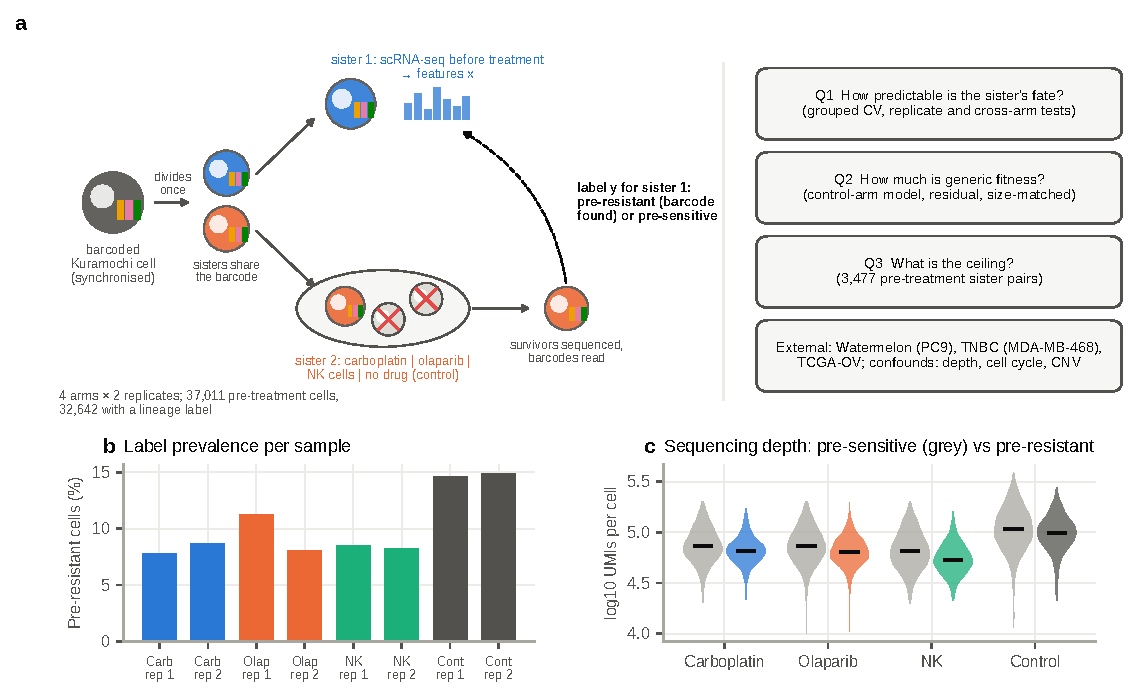
\includegraphics[width=\linewidth]{figures/Fig1_design_data.pdf}
\end{figure*}


\textbf{Figure 1. Study design and data.} (a) ReSisTrace design and the questions addressed in this study. (b) Fraction of labelled pre-treatment cells that are pre-resistant in each sample. (c) UMIs per cell for pre-sensitive (grey) and pre-resistant (coloured) cells in each arm; bars mark medians.

\begin{figure}[htbp]
  \centering
  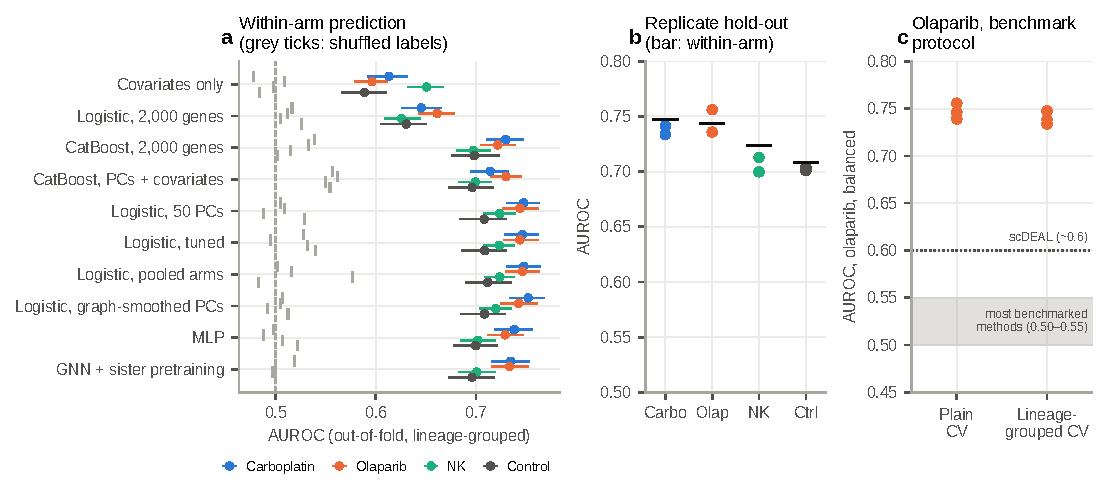
\includegraphics[width=\linewidth]{figures/Fig2_predictability.pdf}
\end{figure}


\textbf{Figure 2. The pre-treatment state predicts a sister's fate.} (a) Out-of-fold AUROC (lineage-grouped five-fold cross-validation) for each model and arm; error bars are 95\% family-bootstrap intervals; grey ticks show the same models retrained on family-level shuffled labels (one to five permutations per model). (b) Replicate hold-out AUROC (dots) for the PCA-logistic model; bars show within-arm AUROC. (c) Olaparib under the benchmark protocol of Shen et al. (2026), with ordinary and lineage-grouped cross-validation (three balanced draws each); the shaded band and dotted line mark the values reported for existing methods in that study.

\begin{figure}[htbp]
  \centering
  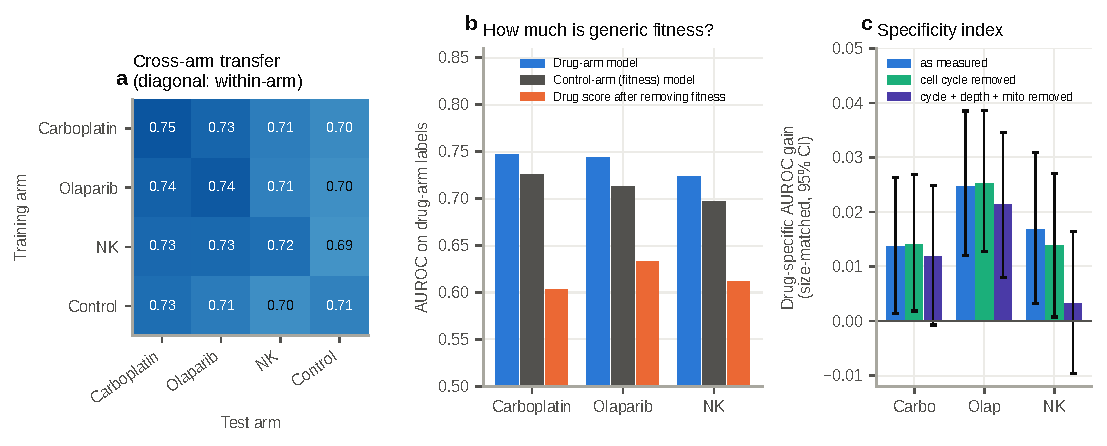
\includegraphics[width=\linewidth]{figures/Fig3_fitness_confound.pdf}
\end{figure}


\textbf{Figure 3. Most of the signal is shared with the untreated control.} (a) AUROC of PCA-logistic models trained on one arm and tested on another; the diagonal shows within-arm cross-validation. (b) For each drug arm: AUROC of the drug-arm model, of the control-arm (fitness) model applied to drug-arm cells, and of the drug score after within-sample regression on the fitness score. (c) Drug-specific AUROC gain over the fitness model with training size matched ($\Delta$AUROC, mean over 10 training subsamples), under three preprocessing variants; error bars are 95\% paired family-bootstrap intervals (Table S19).

\begin{figure}[htbp]
  \centering
  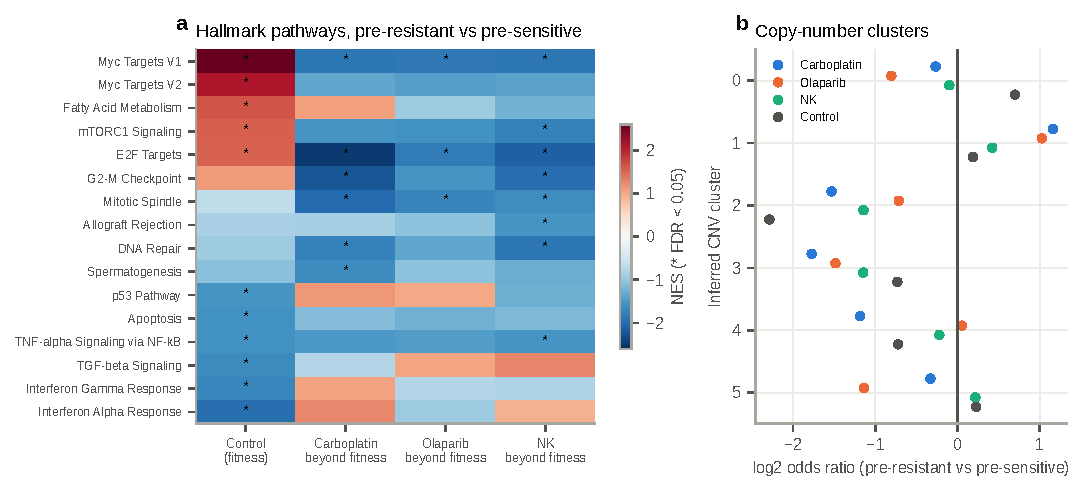
\includegraphics[width=\linewidth]{figures/Fig4_biology.pdf}
\end{figure}


\textbf{Figure 4. Biology of the shared and drug-specific components.} (a) Normalised enrichment scores of Hallmark gene sets for the control contrast (fitness) and for each drug contrast after subtracting the control contrast; asterisks mark FDR $<$ 0.05. (b) Odds ratios for inferred copy-number clusters among pre-resistant versus pre-sensitive cells in each arm.

\begin{figure}[htbp]
  \centering
  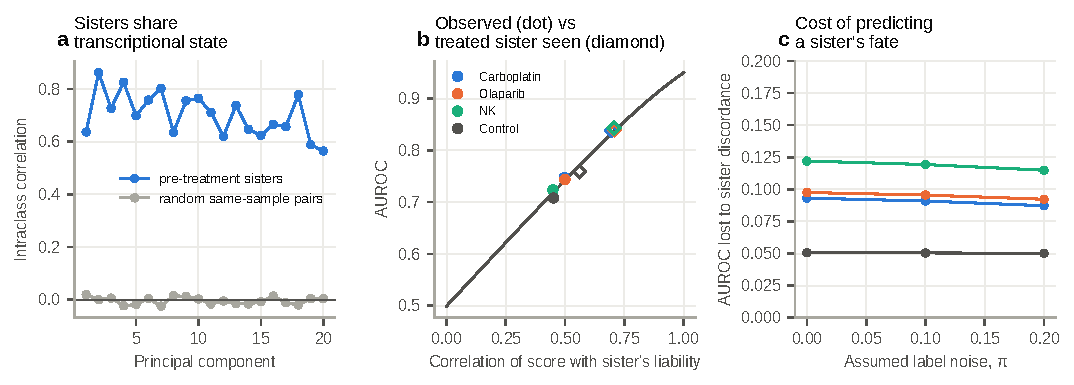
\includegraphics[width=\linewidth]{figures/Fig5_ceiling.pdf}
\end{figure}


\textbf{Figure 5. Sister discordance caps predictability.} (a) Intraclass correlation of principal-component scores between pre-treatment sisters and between random same-sample pairs. (b) Expected AUROC as a function of the correlation between score and sister liability under the bivariate-normal model with label noise $\pi$ = 0.1 (line), with each arm's observed PCA-logistic AUROC (dots) and the AUROC implied if the treated sister's own state were scored (diamonds). (c) AUROC lost to sister discordance as a function of assumed label noise $\pi$.

\begin{figure*}[htbp]
  \centering
  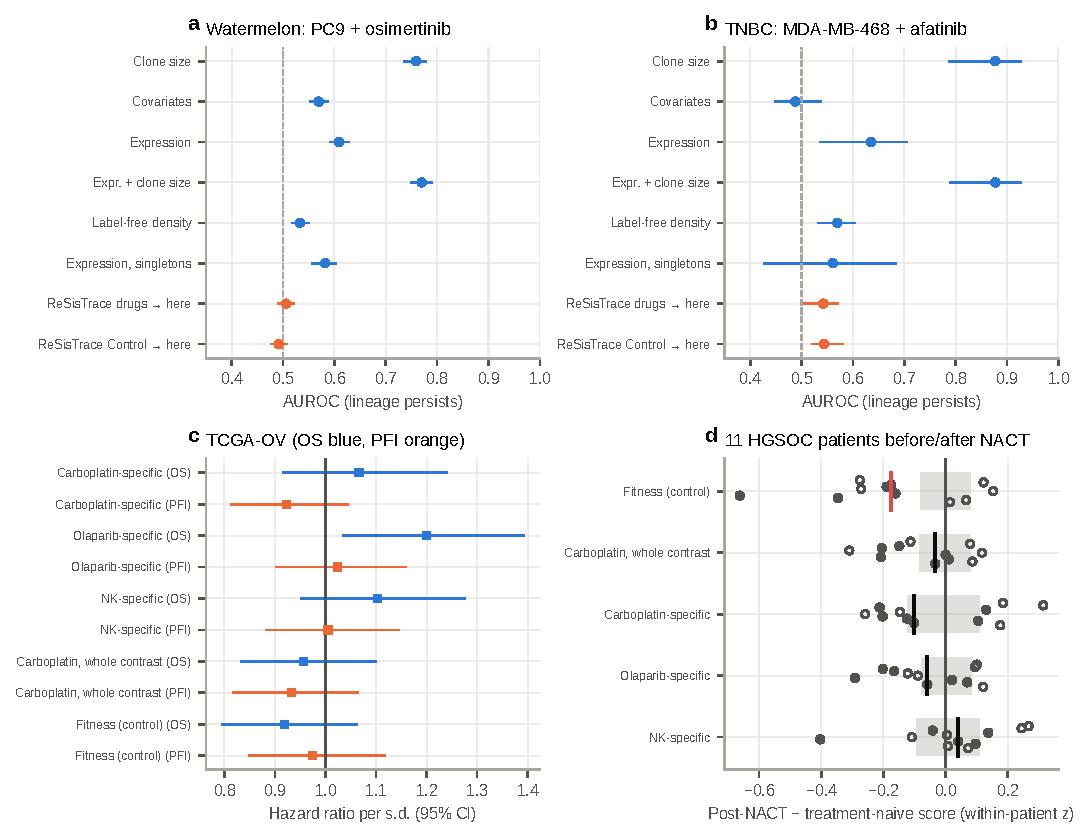
\includegraphics[width=\linewidth]{figures/Fig6_external_clinical.pdf}
\end{figure*}


\textbf{Figure 6. External and clinical checks.} (a, b) AUROC for predicting lineage persistence from untreated cells in Watermelon (a) and triple-negative breast cancer (b), using clone size, technical covariates, expression, the label-free density score, expression within singleton lineages, and zero-shot transfer of ReSisTrace models; error bars are 95\% lineage-bootstrap intervals. (c) Hazard ratios per standard deviation of signature score for overall survival and progression-free interval in TCGA-OV; the fitness, whole-contrast and drug-specific signatures are defined in Methods (Differential expression and pathways). (d) Change in signature score from treatment-naive to post-treatment malignant cells in 11 patients with high-grade serous ovarian cancer receiving neoadjuvant carboplatin--paclitaxel (Zhang et al., 2022); one dot per patient, filled where both samples came from the same anatomical site; the vertical line is the median and the grey band spans $\pm$2 s.d. of the medians of 200 expression-matched random gene sets.

\begin{figure}[htbp]
  \centering
  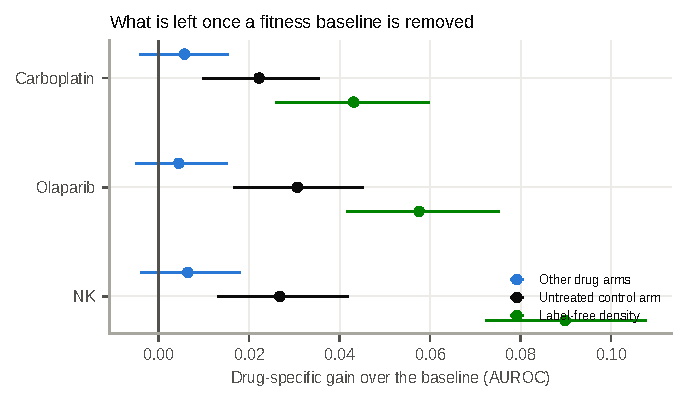
\includegraphics[width=\linewidth]{figures/Fig8_control_free.pdf}
\end{figure}


\textbf{Figure 8. Substitutes for an untreated arm.} For each drug arm of ReSisTrace, the drug-specific gain measured against the real control-arm model (black) and against two substitutes that use no control-arm labels: a model trained on the other drug arms (blue) and the label-free density score (green). Error bars are 95\% family-bootstrap intervals. The control-arm value lies between the two substitutes in every arm.

\begin{figure}[htbp]
  \centering
  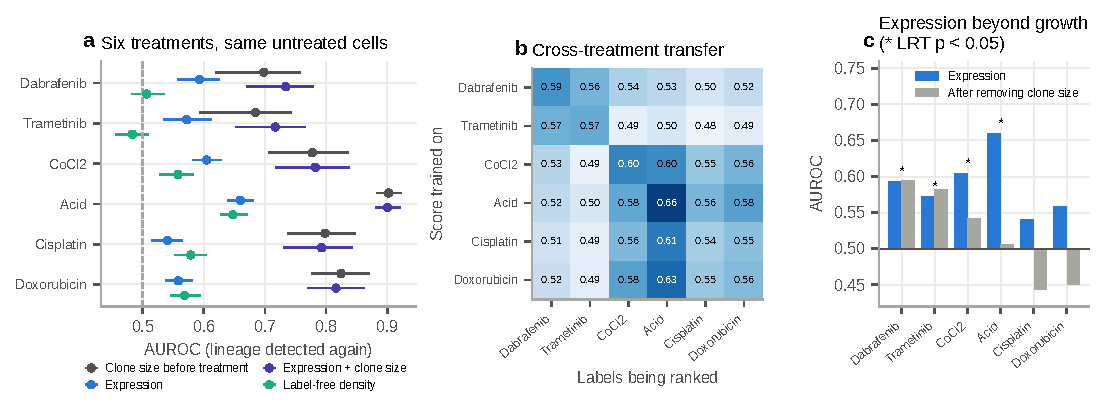
\includegraphics[width=\linewidth]{figures/Fig7_schaff_multitreatment.pdf}
\end{figure}


\textbf{Figure 7. A second lineage system with six treatments (Schaff et al., 2026).} (a) AUROC for predicting whether an untreated cell's lineage is detected again after each treatment, using clone size before treatment, expression (50 principal components), both, and the label-free density score; lineage-grouped cross-validation, error bars are 95\% lineage-bootstrap intervals. (b) AUROC when the out-of-fold score trained on one treatment's labels is used to rank another treatment's labels. (c) Expression AUROC before and after residualising on log clone size, with the likelihood-ratio test for adding expression to clone size.

\begin{figure}[htbp]
  \centering
  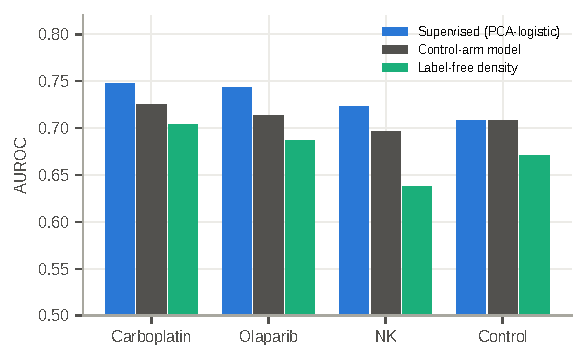
\includegraphics[width=\linewidth]{figures/FigS1_typicality.pdf}
\end{figure}


\textbf{Figure S1. Label-free typicality.} AUROC of the local-density score (negative mean distance to the 15 nearest neighbours within the sample), compared with the supervised PCA-logistic model and the control-arm (fitness) model, for each arm.

\begin{figure}[htbp]
  \centering
  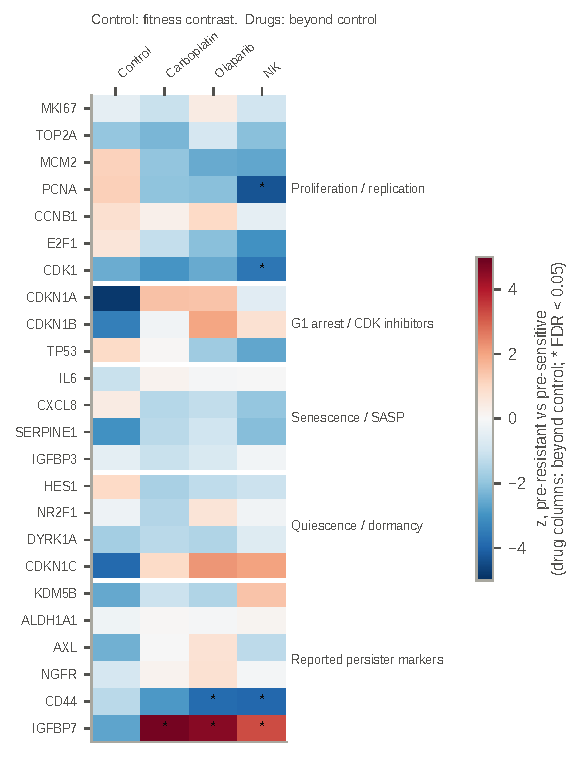
\includegraphics[width=\linewidth]{figures/FigS2_marker_panel.pdf}
\end{figure}


\textbf{Figure S2. Pre-specified marker panel.} z-scores for pre-resistant versus pre-sensitive cells. The control column shows the control (fitness) contrast; the drug columns show the difference from the control contrast, z\_diff = (z\_drug $-$ z\_control)/$\sqrt{2}$. Asterisks mark FDR $<$ 0.05 for z\_diff. Genes not among the 5,005 retained genes (CDKN2A, RB1, GLB1, KDM5A) are omitted.

\begin{figure}[htbp]
  \centering
  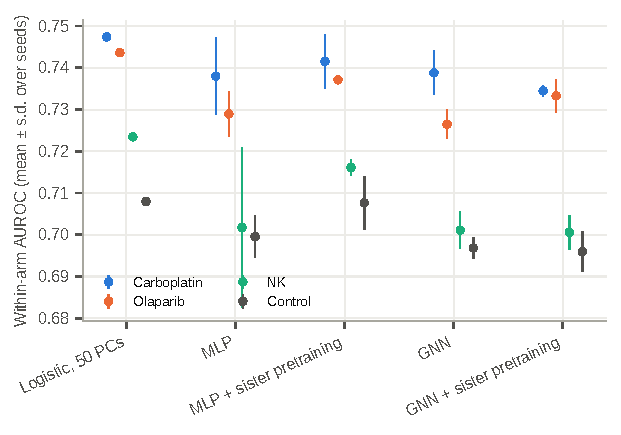
\includegraphics[width=\linewidth]{figures/FigS3_gnn_ablation.pdf}
\end{figure}


\textbf{Figure S3. Graph model ablation.} Within-arm AUROC for logistic regression, an MLP, an MLP with sister-pair pretraining, the graph network, and the graph network with pretraining (mean $\pm$ s.d. over seeds).

\section*{References}

\noindent All references were checked against Europe PMC, NCBI PMC, arXiv, JMLR or Crossref on 25--26 September 2026. For the 29 studies marked , the full text was retrieved and the statements cited above were checked against it; the others were checked against their abstracts.\par\vspace{2pt}

\noindent Aviv H. Pretreatment transcriptional state carries condition-specific information about future clonal detection in a lineage-traced melanoma line. \emph{Zenodo} (2026). doi:10.5281/zenodo.22850050 \par\vspace{2pt}

\noindent Chen H, Venkatesh MS, G\'omez Ortega J, et al. Scaling and quantization of large-scale foundation model enables resource-efficient predictions in network biology. \emph{Nat Comput Sci} 6, 450--463 (2026). doi:10.1038/s43588-026-00972-4\par\vspace{2pt}

\noindent Chen J, Wang X, Ma A, et al. Deep transfer learning of cancer drug responses by integrating bulk and single-cell RNA-seq data. \emph{Nat Commun} 13, 6494 (2022). doi:10.1038/s41467-022-34277-7 \par\vspace{2pt}

\noindent Chen T, Kornblith S, Norouzi M, Hinton G. A simple framework for contrastive learning of visual representations. \emph{ICML} (2020). arXiv:2002.05709\par\vspace{2pt}

\noindent Dai J, Zheng S, Falco MM, et al. Tracing back primed resistance in cancer via sister cells. \emph{Nat Commun} 15, 1158 (2024). doi:10.1038/s41467-024-45478-7 \par\vspace{2pt}

\noindent Davidson-Pilon C. lifelines: survival analysis in Python. \emph{J Open Source Softw} 4, 1317 (2019). doi:10.21105/joss.01317\par\vspace{2pt}

\noindent Emert BL, Cote CJ, Torre EA, et al. Variability within rare cell states enables multiple paths toward drug resistance. \emph{Nat Biotechnol} 39, 865-876 (2021). doi:10.1038/s41587-021-00837-3 \par\vspace{2pt}

\noindent Fang Z, Liu X, Peltz G. GSEApy: a comprehensive package for performing gene set enrichment analysis in Python. \emph{Bioinformatics} 39, btac757 (2023). doi:10.1093/bioinformatics/btac757\par\vspace{2pt}

\noindent Fennell KA, Vassiliadis D, Lam EYN, et al. Non-genetic determinants of malignant clonal fitness at single-cell resolution. \emph{Nature} 601, 125-131 (2022). doi:10.1038/s41586-021-04206-7\par\vspace{2pt}

\noindent Fustero-Torre C, Jim\'enez-Santos MJ, Garc\'ia-Mart\'in S, et al. Beyondcell: targeting cancer therapeutic heterogeneity in single-cell RNA-seq data. \emph{Genome Med} 13, 187 (2021). doi:10.1186/s13073-021-01001-x \par\vspace{2pt}

\noindent Goyal Y, Busch GT, Pillai M, et al. Diverse clonal fates emerge upon drug treatment of homogeneous cancer cells. \emph{Nature} 620, 651-659 (2023). doi:10.1038/s41586-023-06342-8 \par\vspace{2pt}

\noindent Gutierrez C, Al'Khafaji AM, Brenner E, et al. Multifunctional barcoding with ClonMapper enables high-resolution study of clonal dynamics during tumor evolution and treatment. \emph{Nat Cancer} 2, 758-772 (2021). doi:10.1038/s43018-021-00222-8 \par\vspace{2pt}

\noindent Hamilton WL, Ying R, Leskovec J. Inductive representation learning on large graphs. \emph{NeurIPS} (2017). arXiv:1706.02216\par\vspace{2pt}

\noindent Harmange G, Hueros RAR, Schaff DL, et al. Disrupting cellular memory to overcome drug resistance. \emph{Nat Commun} 14, 7130 (2023). doi:10.1038/s41467-023-41811-8 \par\vspace{2pt}

\noindent Hata AN, Niederst MJ, Archibald HL, et al. Tumor cells can follow distinct evolutionary paths to become resistant to epidermal growth factor receptor inhibition. \emph{Nat Med} 22, 262-269 (2016). doi:10.1038/nm.4040 \par\vspace{2pt}

\noindent Iyer A, Alva A, Granada AE, Chakrabarti S. Inheritable cell-states shape drug-persister correlations and population dynamics in cancer cells. \emph{PLoS Comput Biol} 21, e1013446 (2025). doi:10.1371/journal.pcbi.1013446 \par\vspace{2pt}

\noindent Korsunsky I, Millard N, Fan J, et al. Fast, sensitive and accurate integration of single-cell data with Harmony. \emph{Nat Methods} 16, 1289--1296 (2019). doi:10.1038/s41592-019-0619-0\par\vspace{2pt}

\noindent Kronheim S, Wang J, Chen JY, et al. Chemotherapy reshapes cellular clonal landscape via persister programs in breast cancer xenografts. \emph{bioRxiv} (2026). doi:10.64898/2026.04.02.716097 \par\vspace{2pt}

\noindent Lause J, Berens P, Kobak D. Analytic Pearson residuals for normalization of single-cell RNA-seq UMI data. \emph{Genome Biol} 22, 258 (2021). doi:10.1186/s13059-021-02451-7\par\vspace{2pt}

\noindent Liberzon A, Birger C, Thorvaldsd\'ottir H, et al. The Molecular Signatures Database (MSigDB) hallmark gene set collection. \emph{Cell Syst} 1, 417--425 (2015). doi:10.1016/j.cels.2015.12.004\par\vspace{2pt}

\noindent Liu J, Lichtenberg T, Hoadley KA, et al. An integrated TCGA pan-cancer clinical data resource to drive high-quality survival outcome analytics. \emph{Cell} 173, 400--416 (2018). doi:10.1016/j.cell.2018.02.052\par\vspace{2pt}

\noindent Lopez R, Regier J, Cole MB, Jordan MI, Yosef N. Deep generative modeling for single-cell transcriptomics. \emph{Nat Methods} 15, 1053--1058 (2018). doi:10.1038/s41592-018-0229-2\par\vspace{2pt}

\noindent Marine JC, Dawson SJ, Dawson MA. Non-genetic mechanisms of therapeutic resistance in cancer. \emph{Nat Rev Cancer} 20, 743-756 (2020). doi:10.1038/s41568-020-00302-4\par\vspace{2pt}

\noindent Oliveira EA, Milite S, Fernandez-Mateos J, et al. Epigenetic heritability of cell plasticity drives cancer drug resistance through a one-to-many genotype-to-phenotype paradigm. \emph{Cancer Res} 85, 2921-2938 (2025). doi:10.1158/0008-5472.CAN-25-0999 \par\vspace{2pt}

\noindent Oren Y, Tsabar M, Cuoco MS, et al. Cycling cancer persister cells arise from lineages with distinct programs. \emph{Nature} 596, 576-582 (2021). doi:10.1038/s41586-021-03796-6 \par\vspace{2pt}

\noindent Paek AL, Liu JC, Loewer A, et al. Cell-to-Cell Variation in p53 Dynamics Leads to Fractional Killing. \emph{Cell} 165, 631-642 (2016). doi:10.1016/j.cell.2016.03.025 \par\vspace{2pt}

\noindent Patel AP, Tirosh I, Trombetta JJ, et al. Single-cell RNA-seq highlights intratumoral heterogeneity in primary glioblastoma. \emph{Science} 344, 1396-1401 (2014). doi:10.1126/science.1254257 \par\vspace{2pt}

\noindent Pedregosa F, Varoquaux G, Gramfort A, et al. Scikit-learn: machine learning in Python. \emph{J Mach Learn Res} 12, 2825--2830 (2011).\par\vspace{2pt}

\noindent Pellecchia S, Franchini M, Viscido G, et al. Single cell lineage tracing reveals clonal dynamics of anti-EGFR therapy resistance in triple negative breast cancer. \emph{Genome Med} 16, 55 (2024). doi:10.1186/s13073-024-01327-2 \par\vspace{2pt}

\noindent Prokhorenkova L, Gusev G, Vorobev A, Dorogush AV, Gulin A. CatBoost: unbiased boosting with categorical features. \emph{NeurIPS} (2018). arXiv:1706.09516\par\vspace{2pt}

\noindent Ramirez M, Rajaram S, Steininger RJ, et al. Diverse drug-resistance mechanisms can emerge from drug-tolerant cancer persister cells. \emph{Nat Commun} 7, 10690 (2016). doi:10.1038/ncomms10690 \par\vspace{2pt}

\noindent Rehman SK, Haynes J, Collignon E, et al. Colorectal Cancer Cells Enter a Diapause-like DTP State to Survive Chemotherapy. \emph{Cell} 184, 226-242.e21 (2021). doi:10.1016/j.cell.2020.11.018 \par\vspace{2pt}

\noindent Schaff DL, White PE, Cote CJ, et al. Pre-existing cell states predict resistance to multiple treatments. \emph{Cell Genom} 6, 101191 (2026). doi:10.1016/j.xgen.2026.101191 \par\vspace{2pt}

\noindent Shaffer SM, Dunagin MC, Torborg SR, et al. Rare cell variability and drug-induced reprogramming as a mode of cancer drug resistance. \emph{Nature} 546, 431-435 (2017). doi:10.1038/nature22794 \par\vspace{2pt}

\noindent Shaffer SM, Emert BL, Reyes Hueros RA, et al. Memory Sequencing Reveals Heritable Single-Cell Gene Expression Programs Associated with Distinct Cellular Behaviors. \emph{Cell} 182, 947-959.e17 (2020). doi:10.1016/j.cell.2020.07.003 \par\vspace{2pt}

\noindent Sharma SV, Lee DY, Li B, et al. A chromatin-mediated reversible drug-tolerant state in cancer cell subpopulations. \emph{Cell} 141, 69-80 (2010). doi:10.1016/j.cell.2010.02.027 \par\vspace{2pt}

\noindent Shen L, Sun X, Zheng S, et al. Predicting Pre-treatment Resistance or Post-treatment Effect? A Systematic Benchmarking of Single-Cell Drug Response Models. \emph{bioRxiv} (2026), version 2. doi:10.64898/2026.04.10.717709 \par\vspace{2pt}

\noindent Soragni A, Knudsen ES, O'Connor TN, et al. Acquired resistance in cancer: towards targeted therapeutic strategies. \emph{Nat Rev Cancer} 25, 613-633 (2025). doi:10.1038/s41568-025-00824-9 \par\vspace{2pt}

\noindent Spencer SL, Gaudet S, Albeck JG, et al. Non-genetic origins of cell-to-cell variability in TRAIL-induced apoptosis. \emph{Nature} 459, 428-432 (2009). doi:10.1038/nature08012 \par\vspace{2pt}

\noindent Subramanian A, Tamayo P, Mootha VK, et al. Gene set enrichment analysis: a knowledge-based approach for interpreting genome-wide expression profiles. \emph{Proc Natl Acad Sci USA} 102, 15545--15550 (2005). doi:10.1073/pnas.0506580102\par\vspace{2pt}

\noindent Suphavilai C, Chia S, Sharma A, et al. Predicting heterogeneity in clone-specific therapeutic vulnerabilities using single-cell transcriptomic signatures. \emph{Genome Med} 13, 189 (2021). doi:10.1186/s13073-021-01000-y \par\vspace{2pt}

\noindent Theodoris CV, Xiao L, Chopra A, et al. Transfer learning enables predictions in network biology. \emph{Nature} 618, 616--624 (2023). doi:10.1038/s41586-023-06139-9\par\vspace{2pt}

\noindent Tirosh I, Izar B, Prakadan SM, et al. Dissecting the multicellular ecosystem of metastatic melanoma by single-cell RNA-seq. \emph{Science} 352, 189-196 (2016). doi:10.1126/science.aad0501 \par\vspace{2pt}

\noindent Wagner DE, Klein AM. Lineage tracing meets single-cell omics: opportunities and challenges. \emph{Nat Rev Genet} 21, 410-427 (2020). doi:10.1038/s41576-020-0223-2 \par\vspace{2pt}

\noindent Wang SW, Herriges MJ, Hurley K, et al. CoSpar identifies early cell fate biases from single-cell transcriptomic and lineage information. \emph{Nat Biotechnol} 40, 1066-1074 (2022). doi:10.1038/s41587-022-01209-1\par\vspace{2pt}

\noindent Weinreb C, Rodriguez-Fraticelli A, Camargo FD, et al. Lineage tracing on transcriptional landscapes links state to fate during differentiation. \emph{Science} 367, eaaw3381 (2020). doi:10.1126/science.aaw3381 \par\vspace{2pt}

\noindent Wolf FA, Angerer P, Theis FJ. SCANPY: large-scale single-cell gene expression data analysis. \emph{Genome Biol} 19, 15 (2018). doi:10.1186/s13059-017-1382-0\par\vspace{2pt}

\noindent Zhang K, Erkan EP, Jamalzadeh S, et al. Longitudinal single-cell RNA-seq analysis reveals stress-promoted chemoresistance in metastatic ovarian cancer. \emph{Sci Adv} 8, eabm1831 (2022). doi:10.1126/sciadv.abm1831 \par\vspace{2pt}

\noindent Zheng Z, Chen J, Chen X, et al. Enabling Single-Cell Drug Response Annotations from Bulk RNA-Seq Using SCAD. \emph{Adv Sci (Weinh)} 10, e2204113 (2023). doi:10.1002/advs.202204113 \par\vspace{2pt}

\end{document}
